\documentclass[a4paper,14pt]{extarticle}

\usepackage[utf8]{inputenc}
\usepackage[russian]{babel}
\usepackage{graphicx}
\usepackage[top=0.8in, bottom=0.8in, left=0.8in, right=0.8in]{geometry}
\usepackage{pgfplots}
\usepackage{amsmath}
\usepackage{setspace}
\usepackage{titlesec}
\usepackage{float}
\usepackage{chngcntr}
\usepackage{pgfplots}
\usepackage{amsfonts}
\usepackage{pgfplotstable}
\usepackage{multirow}
\usepackage{karnaugh-map}
\usepackage{tikz,xcolor}
\usepackage{listings}

\lstset{ %
extendedchars=\true,
keepspaces=true,
%language=no, % choose the language of the code
basicstyle=\footnotesize, % the size of the fonts that are used for the code
numbers=left, % where to put the line-numbers
numberstyle=\footnotesize, % the size of the fonts that are used for the line-numbers
stepnumber=1, % the step between two line-numbers. If it is 1 each line will be numbered
numbersep=10pt, % how far the line-numbers are from the code
backgroundcolor=\color{white}, % choose the background color. You must add \usepackage{color}
showspaces=false, % show spaces adding particular underscores
showstringspaces=false, % underline spaces within strings
showtabs=false, % show tabs within strings adding particular underscores
frame=single, % adds a frame around the code
tabsize=4, % sets default tabsize to 2 spaces
captionpos=b, % sets the caption-position to bottom
breaklines=true, % sets automatic line breaking
breakatwhitespace=false, % sets if automatic breaks should only happen at whitespace
escapeinside={\%*}{*)}, % if you want to add a comment within your code
%postbreak=\raisebox{0ex}[0ex][0ex]{\ensuremath{\color{red}\hookrightarrow\space}}
}

\titleformat{\section}[hang]
  {\bfseries}
  {}
  {0em}
  {\hspace{-0.4pt}\large \thesection\hspace{0.6em}}
  
  
\titleformat{\subsection}[hang]
  {\bfseries}
  {}
  {0em}
  {\hspace{-0.4pt}\large \thesubsection\hspace{0.6em}}

%\linespread{1.3} % полуторный интервал
%\renewcommand{\rmdefault}{ftm} % Times New Roman

\newcommand{\nx}{\overline{x}}
\newcommand{\p}{0.31}
\newcommand{\scale}{1.4}

\counterwithin{figure}{section}
\counterwithin{equation}{section}
\counterwithin{table}{section}



\begin{document}


\begin{titlepage}
\centering
Санкт-Петербургский политехнический университет Петра Великого \\
\vspace{0.15cm}
Кафедра компьютерных систем и программных технологий \\
\vspace{6.5cm}

{\centering \textbf{Отчёт по лабораторной работе} \\ 
\vspace{0.15cm}
\textbf{Дисциплина}: Разработка сетевых приложений \\
\vspace{0.15cm}
\textbf{Тема}: Изучение прикладных протоколов в командной строке Linux} \\

\vspace{6.5cm}

\begin{table}[H]
\begin{tabular}{p{\textwidth}@{}r}
{Выполнил студент гр. 43501/3} \hfill {Мальцев  М.С.} \\
{Преподаватель} \hfill {Зозуля А.В.} \\
\end{tabular}
\end{table}
\vfill

{\centering Санкт-Петербург \\ 
\vspace{0.15cm}
\today}
\end{titlepage}

\section{SMTP}

\subsection{Основные сведения о протоколе}
Simple Mail Transfer Protocol (SMTP)  - это интернет протокол для обмена почтой. Впервые был зафиксирован в RFC 821 в 1982 году. Был изменен в 2008 году RFC 5321. Используется по сегодняшний день.

\subsection{Основные команды}
Команды SMTP:
\begin{itemize}
\item EHLO - используется для приветствия в протоколе ESMTP. Рекомендуется к использованию по возможности
\item HELO - команда приветствия. Используется для начала сессии
\item MAIL FROM - задается адрес отправителя
\item RCPT TO - указывается получатель
\item DATA - текст сообщения
\item QUIT - выход
\item HELP - списокк доступных команд или описание запрашиваемой команды
\item NOOP - пустая команда, предположительно используется для поддержания соединения
\item RSET - сброс
\end{itemize}

\subsection{Область применения и ограничения протокола}
Простой протокол передачи почты (SMTP), используется для связи с удаленным сервером и последующей отправке сообщений с локального клиента на удаленный сервер, и в конечном итоге на сервер получателя сообщений. На вашем сервере электронной почты, этот процесс контролируется специальной службой (MTA). Стоит упомянуть, что SMTP используется исключительно для отправки сообщений.

Порты SMTP:

    Порт 25 – порт без шифрования
    
    Порт 465 – порт SSL/TLS, также известный как SMTPS

\subsection{Пример использования}
\lstinputlisting {src/1}

\begin{figure}[H]
	\begin{center}
		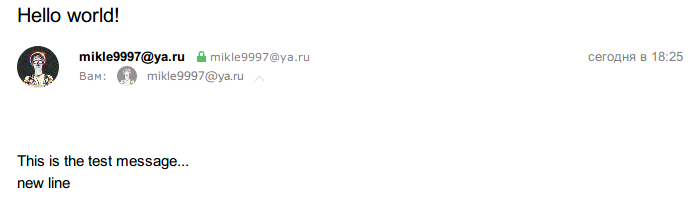
\includegraphics[scale=0.7]{pics/smtp_test.png}
		\caption{Собщение отправленное с использованием протокола smtp}
		\label{clientTCP}
	\end{center}
\end{figure}

\section{POP3}

\subsection{Основные сведения о протоколе}
POP3 (англ. Post Office Protocol Version 3 — протокол почтового отделения, версия 3) — стандартный интернет-протокол прикладного уровня, используемый клиентами электронной почты для получения почты с удалённого сервера по TCP-соединению. 

\subsection{Основные команды}
Команды POP3:
\begin{itemize}
\item USER - передаёт серверу имя пользователя
\item PASS - передаёт серверу пароль почтового ящика.
\item DELE - сервер помечает указанное сообщение для удаления.  Сообщения, помеченные на удаление, реально удаляются только после закрытия транзакции (закрытие транзакций происходит обычно после посыла команды QUIT, кроме этого, например, на серверах закрытие транзакций может происходить по истечении определённого времени, установленного сервером).
\item LIST - если был передан аргумент, то сервер выдаёт информацию об указанном сообщении. Если аргумент не был передан, то сервер выдаёт информацию обо всех сообщениях, находящихся в почтовом ящике. Сообщения, помеченные для удаления, не перечисляются
\item NOOP - сервер ничего не делает, всегда отвечает положительно
\item RETR сообщение - сервер передаёт сообщение с указанным номером
\item RSET - этой командой производится откат транзакций внутри сессии. Например, если пользователь случайно пометил на удаление какие-либо сообщения, он может убрать эти пометки, отправив эту команду
\item STAT -сервер возвращает количество сообщений в почтовом ящике и размер почтового ящика в октетах. Сообщения, помеченные как удалённые, при этом не учитываются. 
\item TOP - сервер возвращает заголовки указанного сообщения, пустую строку и указанное количество первых строк тела сообщения.
\end{itemize}

\subsection{Область применения и ограничения протокола}
POP3 (протокол почтового отделения версия 3) часто используется для связи с удаленным сервером электронной почты и загрузки сообщений на локальный почтовый клиент с последующим удалением его на сервере, к примеру Outlook, Thunderbird, Windows Mail, Mac Mail и т.д. Однако обычно почтовые клиенты предлагают выбор – оставлять или нет копии сообщений на сервере. Если вы используете несколько устройств для отправки сообщений, то рекомендуется оставлять эту функцию включенной, в противном случае, на другом устройстве у вас не будет доступа к отправленным сообщениям, которые не были сохранены на удаленном сервере. Также стоит отметить, что POP3 – протокол работающий только в одном направлении, это означает, что данные берутся с удаленного сервера и отправляются на локальный клиент.

Порты POP3, по умолчанию являются такими:

Порт 110 – порт без шифрования

Порт 995 – порт SSL/TLS, также известный как POP3S

\subsection{Пример использования}
\lstinputlisting {src/2}

\section{IMAP}

\subsection{Основные сведения о протоколе}
IMAP (англ. Internet Message Access Protocol) — протокол прикладного уровня для доступа к электронной почте.

IMAP предоставляет пользователю обширные возможности для работы с почтовыми ящиками, находящимися на центральном сервере. Почтовая программа, использующая этот протокол, получает доступ к хранилищу корреспонденции на сервере так, как будто эта корреспонденция расположена на компьютере получателя. Электронными письмами можно манипулировать с компьютера пользователя (клиента) без постоянной пересылки с сервера и обратно файлов с полным содержанием писем. 

\subsection{Основные команды}
Команды IMAP:
\begin{itemize}
\item LOGIN - позволяет клиенту при регистрации на сервере IMAP использовать идентификатор пользователя и пароль в обычном текстовом виде. Это не самый лучший метод, но иногда это единственная возможность подключиться к серверу
\item CLOSE - закрывает почтовый ящик. Когда почтовый ящик закрыт с помощью этой команды, то сообщения, помеченные флагом DELETED, удаляются из него. Не имеет параметров
\item LOGOUT - завершает сеанс для текущего идентификатора пользователя
\item DELETE - применяется к почтовым ящикам. Сервер IMAP при получении этой команды попытается удалить почтовый ящик с именем, указанным в качестве аргумента команды. Сообщения удаляются вместе с ящиками и восстановлению не подлежат
\item LIST - получить список всех почтовых ящиков клиента; имеет два параметра
\item LSUB - в отличие от команды LIST используется для получения списка ящиков, активизированных командой SUBSCRIBE. Параметры — такие же, как у LIST
\item EXPUNGE - удаляет из почтового ящика все сообщения, помеченные флагом DELETED, при этом почтовый ящик не закрывается. Ответ сервера на команду EXPUNGE представляет собой отчёт о новом состоянии почтового ящика
\item FETCH - получить текст почтового сообщения. Команда применяется только для отображения сообщений. В отличие от POP3, клиент IMAP не сохраняет копию сообщения на клиентском ПК
\item SEARCH - поиск сообщений по критериям в активном почтовом ящике с последующим отображением результатов в виде номера сообщения. Возможен поиск сообщений, в теле которых имеется определённая текстовая строка, или имеющих определённый флаг, или полученных до определённой даты и т.д.
\item NOOP - команда ничего не делает
\end{itemize}

\subsection{Область применения и ограничения протокола}
IMAP, также как и POP3 используется для получения сообщений электронной почты на локальный клиент, однако, он имеет существенное отличие – загружаются только лишь заголовки электронных сообщений, сам текст письма остается на сервере. Данный протокол связи работает в две стороны, если происходят изменения на локальном клиенте, они передаются и на сервер. В последнее время IMAP стал более популярным, так как такие гиганты-провайдеры услуг электронной почты, как Gmail, стали рекомендовать использовать его вместо POP3.

Для отправки писем используется обычно протокол SMTP, так как собственная команда отправки протокола IMAP, называемая APPEND, считается «неудачной» и «небезопасной»

Порты IMAP, по умолчанию являются такими:

    Порт 143 – порт без шифрования
    
    Порт 993 – порт SSL/TLS, также известный как IMAPS

\subsection{Пример использования}
\lstinputlisting {src/3}

\section{HTTP}

\subsection{Основные сведения о протоколе}
HTTP (англ. HyperText Transfer Protocol — «протокол передачи гипертекста») — протокол прикладного уровня передачи данных. Изначально — в виде гипертекстовых документов в формате «HTML», в настоящий момент используется для передачи произвольных данных. 

\subsection{Основные команды}
Команды HTTP:
\begin{itemize}
\item OPTIONS - используется для определения возможностей веб-сервера или параметров соединения для конкретного ресурса
\item GET - используется для запроса содержимого указанного ресурса
\item HEAD - аналогичен методу GET, за исключением того, что в ответе сервера отсутствует тело
\item POST - применяется для передачи пользовательских данных заданному ресурсу
\item PUT - применяется для загрузки содержимого запроса на указанный в запросе URI
\item DELETE - удаляет указанный ресурс
\end{itemize}

\subsection{Область применения и ограничения протокола}
HTTP — протокол прикладного уровня; аналогичными ему являются FTP и SMTP. Обмен сообщениями идёт по обыкновенной схеме «запрос-ответ». Для идентификации ресурсов HTTP использует глобальные URI. В отличие от многих других протоколов, HTTP не сохраняет своего состояния. Это означает отсутствие сохранения промежуточного состояния между парами «запрос-ответ». Компоненты, использующие HTTP, могут самостоятельно осуществлять сохранение информации о состоянии, связанной с последними запросами и ответами (например, «куки» на стороне клиента, «сессии» на стороне сервера). Браузер, посылающий запросы, может отслеживать задержки ответов. Сервер может хранить IP-адреса и заголовки запросов последних клиентов. Однако сам протокол не осведомлён о предыдущих запросах и ответах, в нём не предусмотрена внутренняя поддержка состояния, к нему не предъявляются такие требования. 

\subsection{Пример использования}
\lstinputlisting {src/4}

\section{FTP}

\subsection{Основные сведения о протоколе}
FTP (англ. File Transfer Protocol) — протокол передачи файлов по сети. Гарантирует передачу (либо выдачу ошибки) за счёт применения квитируемого протокола TCP.FTP является одним из старейших прикладных протоколов, появившимся задолго до HTTP, и даже до TCP/IP, в 1971 году. В первое время он работал поверх протокола NCP. Он и сегодня широко используется для распространения ПО и доступа к удалённым хостам. 

\subsection{Основные команды}
Команды FTP:
\begin{itemize}
\item ABOR — прервать передачу файла
\item CDUP — сменить каталог на вышестоящий
\item CWD — сменить каталог
\item DELE — удалить файл (DELE filename)
\item EPSV — войти в расширенный пассивный режим. Применяется вместо PASV
\item HELP — выводит список команд, принимаемых сервером
\item LIST — возвращает список файлов каталога. Список передаётся через соединение данных
\item MDTM — возвращает время модификации файла
\item MKD — создать каталог
\item NLST — возвращает список файлов каталога в более кратком формате, чем LIST. Список передаётся через соединение данных
\item NOOP — пустая операция
\item PASS — пароль
\item PASV — войти в пассивный режим. Сервер вернёт адрес и порт, к которому нужно подключиться, чтобы забрать данные. Передача начнётся при введении следующих команд: RETR, LIST и т.д.
\item PORT — войти в активный режим. Например PORT 12,34,45,56,78,89. В отличие от пассивного режима для передачи данных сервер сам подключается к клиенту
\item PWD — возвращает текущий каталог
\item QUIT — отключиться
\item REIN — реинициализировать подключение
\item RETR — скачать файл. Перед RETR должна быть команда PASV или PORT
\item RMD — удалить каталог
\item RNFR и RNTO — переименовать файл. RNFR — что переименовывать, RNTO — во что
\item SIZE — возвращает размер файла
\item STOR — закачать файл. Перед STOR должна быть команда PASV или PORT
\item SYST — возвращает тип системы (UNIX, WIN, …)
\item TYPE — установить тип передачи файла (бинарный, текстовый)
\item USER — имя пользователя для входа на сервер
\end{itemize}

\subsection{Область применения и ограничения протокола}
Типичное применение FTP-протокола — загрузка сайтов и других документов с частного устройства разработки на общедоступные сервера хостинга. Протокол FTP (как и HTTP) имеет двоичный режим передачи, что сокращает накладные расходы трафика и уменьшает время обмена данными при передаче больших файлов. 

Стандартный порт управления FTP-соединением — 21.

\subsection{Пример использования}
\lstinputlisting {src/5}

При помощи утилиты telnet загрузить файл с FTP-сервера ftp.sunet.se

\section{TFTP}

\subsection{Основные сведения о протоколе}
TFTP (англ. Trivial File Transfer Protocol — простой протокол передачи файлов) используется главным образом для первоначальной загрузки бездисковых рабочих станций. TFTP, в отличие от FTP, не содержит возможностей аутентификации (хотя возможна фильтрация по IP-адресу) и основан на транспортном протоколе UDP. 

\subsection{Основные команды}
Сначала в TFTP-пакете идет поле размером в 2 байта, определяющее тип пакета:
\begin{itemize}
\item Read Request (RRQ, 1) — запрос на чтение файла
\item Write Request (WRQ, 2) — запрос на запись файла
\item Data (DATA, 3) — данные, передаваемые через TFTP
\item Acknowledgment (ACK, 4) — подтверждение пакета
\item Error (ERR, 5) — ошибка
\item Option Acknowledgment (OACK, 6) — подтверждение опций
\end{itemize}
    
\subsection{Область применения и ограничения протокола}
Основное назначение TFTP — обеспечение простоты реализации клиента. В связи с этим он используется для загрузки бездисковых рабочих станций, загрузки обновлений и конфигураций в «умные» сетевые устройства, записи статистики с мини-АТС (CDR) и аппаратных маршрутизаторов/файрволов.

Порт 69.

\subsection{Пример использования}
\lstinputlisting {src/6}

При помощи утилиты netcat выяснить имя файла, который запрашивает удаленный хост (припомощи утилиты tftp) у данного хоста

\section{WebDAV}

\subsection{Основные сведения о протоколе}
WebDAV (Web Distributed Authoring and Versioning) или просто DAV — набор расширений и дополнений к протоколу HTTP, поддерживающих совместную работу пользователей над редактированием файлов и управление файлами на удаленных веб-серверах. В качестве миссии рабочей группы по созданию DAV было заявлено: "разработка дополнений к протоколу HTTP, обеспечивающих свободное взаимодействие инструментов распределенной разработки веб-страниц, в соответствии с потребностями работы пользователей". Однако в процессе эксплуатации DAV нашёл себе ряд других применений, выходящих за первоначально принятые рамки коллективной работы над веб-документами.

\subsection{Основные команды}
WebDAV расширяет HTTP следующими методами запроса:
\begin{itemize}
\item PROPFIND — Получение свойств объекта на сервере в формате XML. Также можно получать структуру репозитория (дерево каталогов);
\item PROPPATCH — Изменение свойств за одну транзакцию;
\item MKCOL — Создать коллекцию объектов (каталог в случае доступа к файлам);
\item COPY — Копирование из одного URI в другой;
\item MOVE — Перемещение из одного URI в другой;
\item LOCK — Поставить блокировку на объекте. WebDAV поддерживает эксклюзивные и общие (shared) блокировки;
\item UNLOCK — Снять блокировку с ресурса.
\end{itemize}
   
\subsection{Область применения и ограничения протокола}
Сегодня DAV применяется в качестве сетевой файловой системы, эффективной для работы в Интернете и способной обрабатывать файлы целиком, поддерживая хорошую производительность работы в условиях окружения с высокой временной задержкой передачи информации. Кроме того, DAV широко применяется в качестве протокола для доступа через Интернет и манипулирования содержимым систем документооборота (document management system). Ещё одной важной целью DAV является поддержка работы распределенных команд по разработке программного обеспечения. В качестве резюме задачу создания DAV можно указать так: на волне повсеместного использования HTTP в качестве стандартного уровня доступа к широкому кругу хранилищ информации расширить его возможности средствами записи информации (HTTP — доступ на чтение, DAV — доступ на запись). 

\subsection{Пример использования}
\lstinputlisting {src/7}

При помощи утилиты curl загрузить файл, создать директорию, выгрузить файл на сервисdisk.yandex.ru.


\section{Вывод}
В ходе работы были использованы следующие протоколы: SMTP, POP3, IMAP, HTTP, FTP, TFTP, WebDAV.

Учитывая имеющиеся теоретические знания о работе рассматриваемых протоколов и небольшой опыт их использования, проделанная работа позволяет лучше проникнуться тонкостями работы с почтовыми серверами и веб-сервисами. В итоге работы были получены навыки и укреплены знания, благодаря которым разработка приложений с использованием рассматриваемых протоколов не вызовет больших сложностей. 

Выполнение подобных заданий явялется полезным и необходимым действием перед написанием собственного приложения использующего указанные протоколы.


\end{document}
